
% v2-acmsmall-sample.tex, dated March 6 2012
% This is a sample file for ACM small trim journals
%
% Compilation using 'acmsmall.cls' - version 1.3 (March 2012), Aptara Inc.
% (c) 2010 Association for Computing Machinery (ACM)
%
% Questions/Suggestions/Feedback should be addressed to => "acmtexsupport@aptaracorp.com".
% Users can also go through the FAQs available on the journal's submission webpage.
%
% Steps to compile: latex, bibtex, latex latex
%
% For tracking purposes => this is v1.3 - March 2012
\documentclass[prodmode,acmtecs]{acmsmall} % Aptara syntax
\usepackage[spanish,polish]{babel}
\usepackage[T1]{fontenc}
\usepackage{fancyvrb}
\usepackage{graphicx,hyperref}
\newcommand\cutout[1]{}


\usepackage[table]{xcolor}
\usepackage[utf8]{inputenc}
\usepackage[parfill]{parskip}
\usepackage{tabulary}
\PassOptionsToPackage{hyphens}{url}
\usepackage{hyperref}    
\usepackage[capitalize]{cleveref}


% Metadata Information
% !!! TODO: SET THESE VALUES !!!
\acmVolume{0}
\acmNumber{0}
\acmArticle{CFP}
\acmYear{0}
\acmMonth{0}

\newcounter{colstart}
\setcounter{page}{4}

\RecustomVerbatimCommand{\VerbatimInput}{VerbatimInput}%
{
%fontsize=\footnotesize,
fontfamily=\rmdefault
}


\newcommand{\UnderscoreCommands}{%\do\verbatiminput%
\do\citeNP \do\citeA \do\citeANP \do\citeN \do\shortcite%
\do\shortciteNP \do\shortciteA \do\shortciteANP \do\shortciteN%
\do\citeyear \do\citeyearNP%
}

\usepackage[strings]{underscore}



% Document starts
\begin{document}


\setcounter{colstart}{\thepage}

\acmArticle{CFP}
\title{\huge\sc SIGLOG Monthly 223}
\author{DAVID PURSER\affil{Max Planck Institute for Software Systems, Saarbr\"ucken}
\vspace*{-2.6cm}\begin{flushright}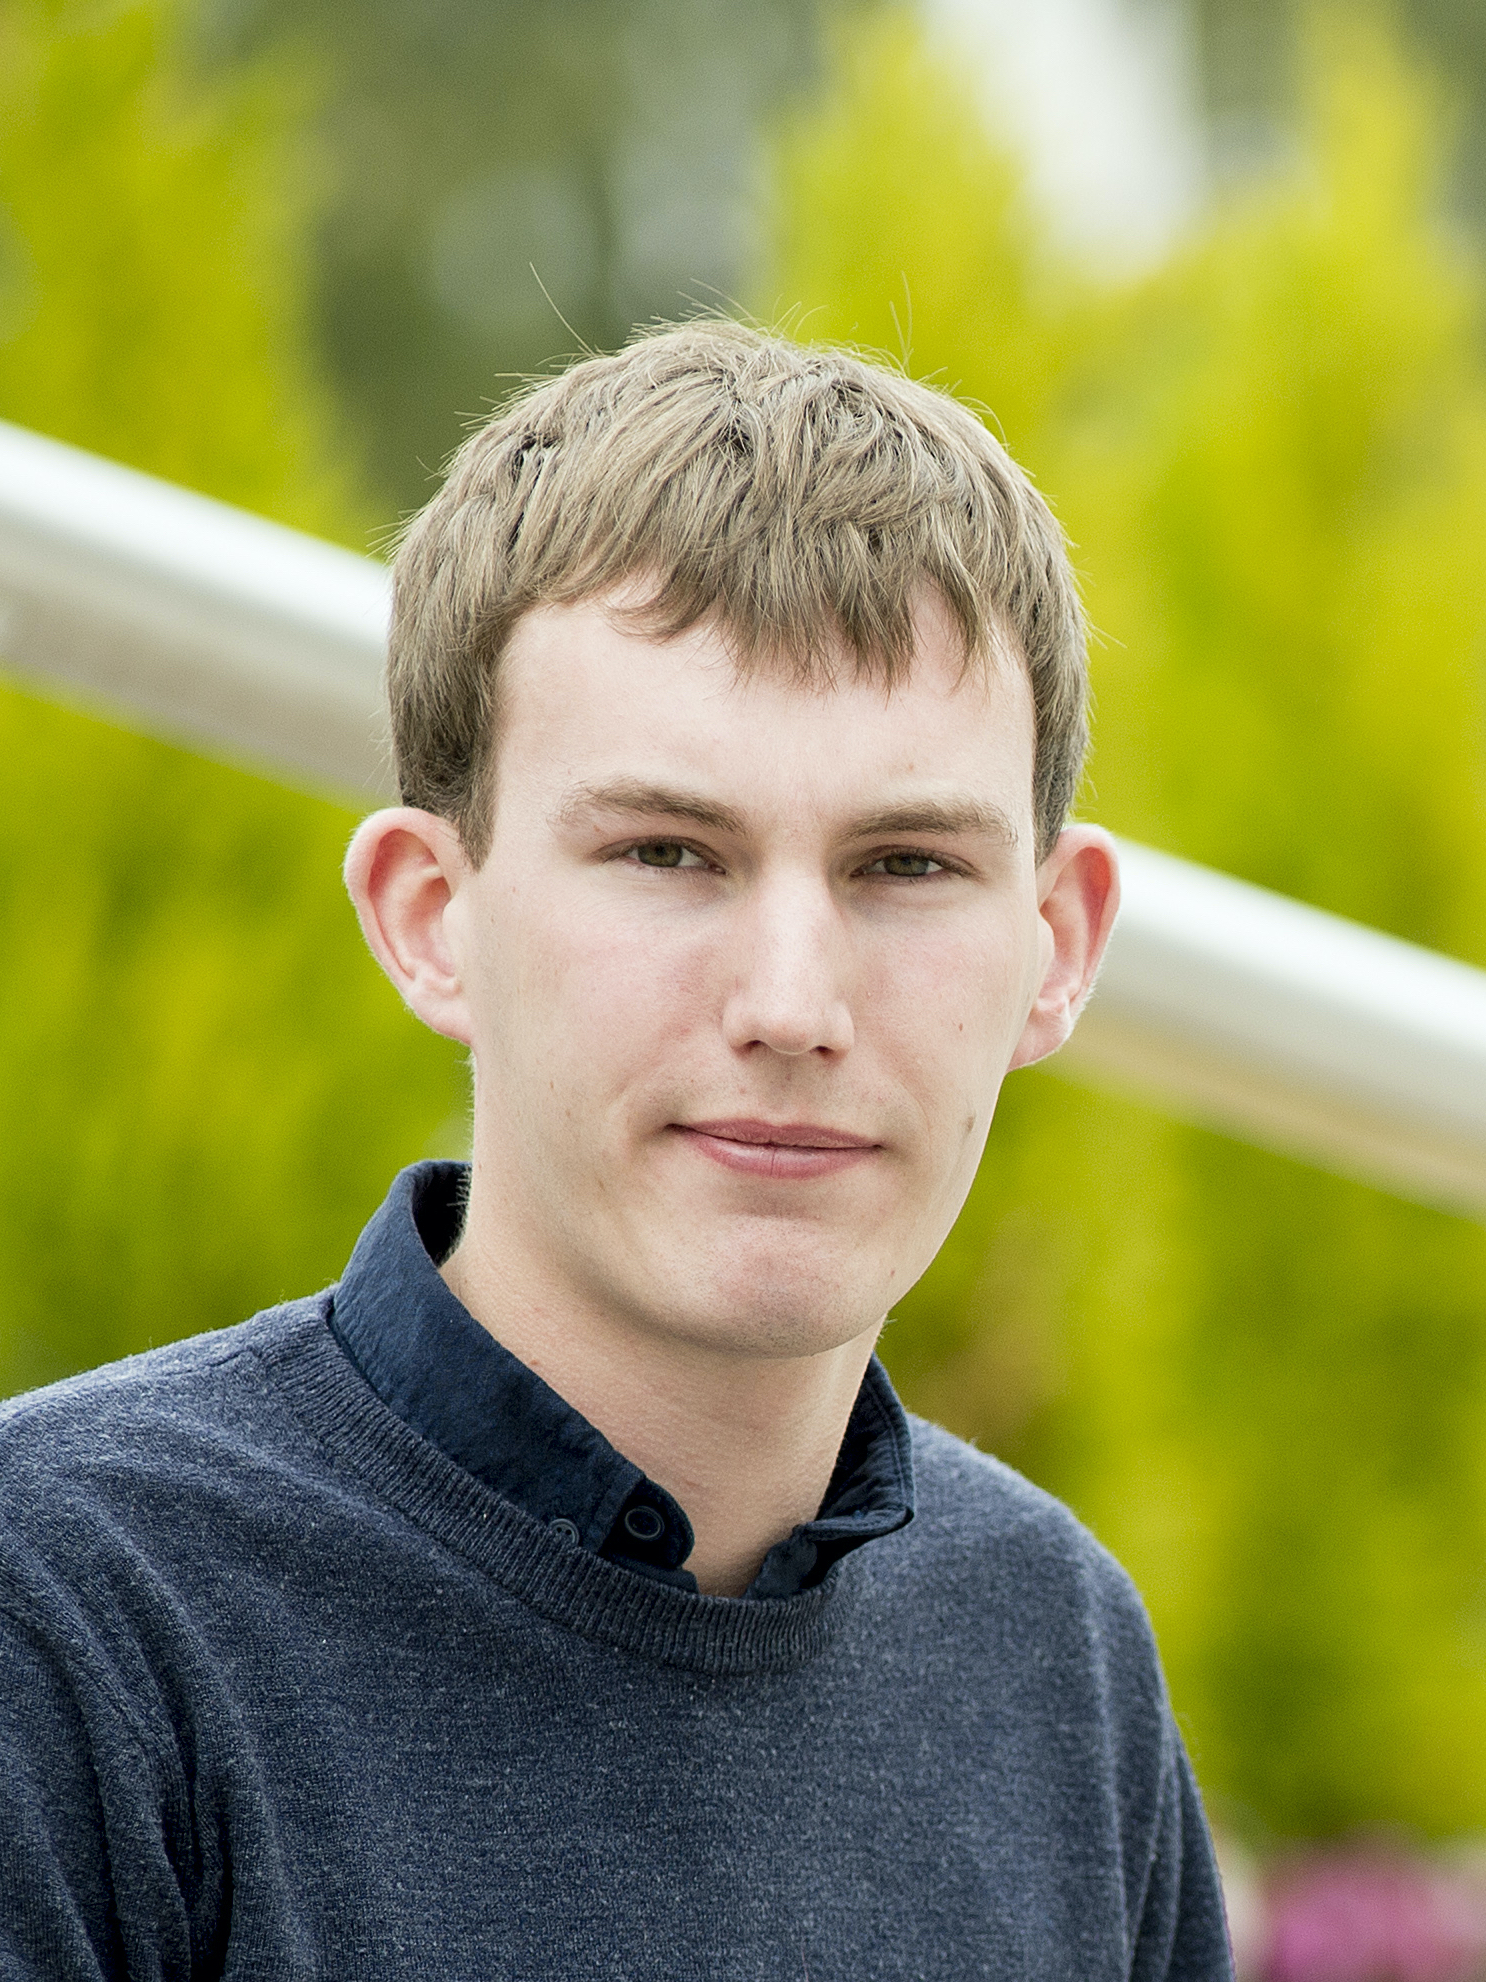
\includegraphics[width=30mm]{dp}\end{flushright}
}

\maketitlee

\href{https://lics.siglog.org/newsletters/}{Past Issues}
 - 
\href{https://lics.siglog.org/newsletters/inst.html}{How to submit an announcement}
\section{Table of Content}\begin{itemize}\item DEADLINES (\cref{deadlines}) 
 
\item SIGLOG MATTERS 
 
\begin{itemize}\item 2022 SIGLOG ELECTIONS (\cref{2022SIGLOGELECTIONS})
\item The 2022 Alonzo Church Award for Outstanding Contributions to Logic and Computation (\cref{The2022AlonzoChurchAwardforOutstandingContributionstoLogicandComputation})
\end{itemize} 
\item CALLS 
 
\begin{itemize}\item ACM PODS 2022 ALBERTO O. MENDELZON TEST-OF-TIME AWARD (CALL FOR NOMINATIONS) (\cref{ACMPODS2022ALBERTOOMENDELZONTESTOFTIMEAWARD})
\item SPIN 2022 (CALL FOR PAPERS) (\cref{SPIN2022})
\item GCM 2022 (CALL FOR PAPERS) (\cref{GCM2022})
\item DECFOML (CALL FOR CONTRIBUTIONS) (\cref{DECFOML})
\item WPTE 2022 (CALL FOR PAPERS) (\cref{WPTE2022})
\item MOVEP2022 (CALL FOR PARTICIPATION) (\cref{MOVEP2022})
\item ASL 2022 (CALL FOR PAPERS) (\cref{ASL2022})
\item NSV 2022 (CALL FOR CONTRIBUTIONS) (\cref{NSV2022})
\item PODS 2023 (CALL FOR RESEARCH PAPERS) (\cref{PODS2023})
\item ACKERMANN AWARD 2022 (CALL FOR NOMINATIONS) (\cref{ACKERMANNAWARD2022})
\end{itemize} 
\item JOB ANNOUNCEMENTS 
 
\begin{itemize}\item Post-doc/senior researcher in smart contract security analysis using formal methods. (\cref{Postdocseniorresearcherinsmartcontractsecurityanalysisusingformalmethods})
\end{itemize} 
\end{itemize}\section{Deadlines}\label{deadlines}\rowcolors{1}{white}{gray!25}\begin{tabulary}{\linewidth}{LL}AiML 2022:  & Mar 07, 2022 (Abstracts for full papers), Mar 14, 2022 (Full papers), May 23, 2022 (Short presentations) \\
TYPES 2022 and CA20111:  & Mar 09, 2022 (2 page abstract) \\
PODS 2022:  & Mar 15, 2022 (Nominations for Test-of-Time Award) \\
SPIN 2022:  & Mar 25, 2022 (Paper s) \\
LearnAut:  & Mar 31, 2022 (Submission deadline) \\
Alonzo Church Award:  & Apr 02, 2022 (Deadline for nominations) \\
NALOMA 22:  & Apr 15, 2022 (Papers \& extended abstracts) \\
FORMATS 2022:  & Apr 19, 2022 (Abstract), Apr 22, 2022 (Paper) \\
GCM 2022:  & Apr 20, 2022 (Abstract Submission), Apr 27, 2022 (Paper Submission) \\
DECFOML:  & Apr 22, 2022 (Submissions) \\
LPNMR 2022:  & Apr 23, 2022 (Paper registration), Apr 30, 2022 (Paper) \\
WPTE 2022:  & Apr 26, 2022 (Abstract), May 03, 2022 (Paper) \\
ATVA 2022:  & May 01, 2022 (Abstract, extended), May 08, 2022 (Paper, extended) \\
MOVEP2022:  & May 01, 2022 (Sudent Abstract), Apr 30, 2022 (Early registration deadline) \\
ASL 2022:  & May 10, 2022 (Papers) \\
NSV 2022:  & May 10, 2022 (Paper) \\
PODS 2023:  & May 30, 2022 (First cycle abstract), Jun 06, 2022 (Full paper), Nov 28, 2022 (Second cycle abstract), Dec 05, 2022 (Full paper) \\
ACKERMANN AWARD 2022:  & Jul 01, 2022 (Deadline for nomination) \\
\end{tabulary}
\section{2022 SIGLOG ELECTIONS}\label{2022SIGLOGELECTIONS}SIGLOG MATTER 

\begin{itemize}\item  Every three years SIGLOG elects new office holders, these are: Chair, Vice-chair, Treasurer and Secretary. SIGLOG will hold elections in April 2022. Only SIGLOG members can vote. The current slate is available at \href{https://www.acm.org/elections/sigs/2022-candidate-slate}{https://www.acm.org/elections/sigs/2022-candidate-slate}.  
 
\item  In accordance with SIG Bylaws, additional candidates may be placed on the ballot by petition. All candidates must be ACM Professional Members, as well as members of SIGLOG. Anyone interested in petitioning must inform ACM Headquarters, Pat Ryan (ryanp@hq.acm.org) and the current Secretary of SIGLOG, Andrzej Murawski (andrzej.murawski@cs.ox.ac.uk) of their intent to petition by 15 March 2022. Petitions must be submitted to ACM Headquarters for verification by 1 April 2022. Further information about SIG elections can be found at \href{https://www.acm.org/elections/sigs/pol_proc}{https://www.acm.org/elections/sigs/pol\_proc}.  
 
\end{itemize}\section{The 2022 Alonzo Church Award for Outstanding Contributions to Logic and Computation}\label{The2022AlonzoChurchAwardforOutstandingContributionstoLogicandComputation}CALL FOR NOMINATIONS 

\begin{itemize}\item  INTRODUCTION 
 
  An annual award, called the Alonzo Church Award for Outstanding Contributions to Logic and Computation, was established in 2015 by the ACM Special Interest Group for Logic and Computation (SIGLOG), the European Association for Theoretical Computer Science (EATCS), the European Association for Computer Science Logic (EACSL), and the Kurt Goedel Society (KGS). The award is for an outstanding contribution represented by a paper or by a small group of papers published within the past 25 years. This time span allows the lasting impact and depth of the contribution to have been established. The award can be given to an individual, or to a group of individuals who have collaborated on the research. For the rules governing this award, see \href{https://siglog.org/alonzo-church-award/}{https://siglog.org/alonzo-church-award/}, \href{https://www.eatcs.org/index.php/church-award/}{https://www.eatcs.org/index.php/church-award/}, and \href{https://www.eacsl.org/alonzo-church-award/}{https://www.eacsl.org/alonzo-church-award/}. 
 
  The 2021 Alonzo Church Award was given jointly to Georg Gottlob, Christoph Koch, Reinhard Pichler, Luc Segoufin and Klaus U. Schulz for their ground-breaking work on logic-based web-data extraction, and querying tree-structured data. Lists containing this and all previous winners can be found through the links above.  
 
\item  ELIGIBILITY AND NOMINATIONS 
 
  The contribution must have appeared in a paper or papers published within the past 25 years. Thus, for the 2022 award, the cut-off date is January 1, 1997. When a paper has appeared in a conference and then in a journal, the date of the journal publication will determine the cut-off date. In addition, the contribution must not yet have received recognition via a major award, such as the Turing Award, the Kanellakis Award, or the Goedel Prize. (The nominee(s) may have received such awards for other contributions.) While the contribution can consist of conference or journal papers, journal papers will be given a preference. 
 
  Nominations for the 2022 award are now being solicited. The nominating letter must summarize the contribution and make the case that it is fundamental and outstanding. The nominating letter can have multiple co-signers. Self-nominations are excluded. Nominations must include: a proposed citation (up to 25 words); a succinct (100-250 words) description of the contribution; and a detailed statement (not exceeding four pages) to justify the nomination. Nominations may also be accompanied by supporting letters and other evidence of worthiness. 
 
  Nominations should be submitted to rjagadee@depaul.edu by April 2, 2022. 
 
\item  PRESENTATION OF THE AWARD 
 
  The 2022 award will be presented at the Federated Logic Conference 2022, which is scheduled to take place in Haifa, Israel in July/August 2022. The award will be accompanied by an invited lecture by the award winner, or by one of the award winners. The awardee(s) will receive a certificate and a cash prize of USD 2,000. If there are multiple awardees, this amount will be shared. 
 
\item  AWARD COMMITTEE 
 
  The 2022 Alonzo Church Award Committee consists of the following five members: Thomas Colcombet, Mariangiola Dezani, Javier Esparza, Radha Jagadeesan (chair), and Igor Walukiewicz. 
 
\end{itemize}\section{ACM PODS 2022 ALBERTO O. MENDELZON TEST-OF-TIME AWARD}\label{ACMPODS2022ALBERTOOMENDELZONTESTOFTIMEAWARD}CALL FOR NOMINATIONS 

\begin{itemize}\item  Nominations are solicited for the PODS 2022 Test-of-Time Award. The award will recognize a paper or a small number of papers published in the PODS 2012 proceedings that had the most impact in terms of research,methodology, or transfer to practice over the intervening decade. 
 
  All papers are nominated by default, but the committee welcomes input from our community. Please feel free to nominate a paper if you think it has had great impact, even if you have not thoroughly compared it to the other eligible papers. The usual conflict of interest rules apply. 
 
\item  The PODS 2022 Test-of-Time Award Committee consists of Michael Bender, Michael Benedikt (chair), and Sudeepa Roy 
 
  Please email your nominations to Michael (michael.benedikt@cs.ox.ac.uk) with subject line ``PODS 2022 ToT Award nomination'' together with a brief justification.  
 
  Please send your nominations no later than March 15, 2022.Nominations are confidential and will only be shared among the committee members. 
 
  The PODS Test-of-Time Award for 2022 will be presented during the SIGMOD/PODS Joint Conference held June 12- June 19, 2022 in Philadelphia, USA . The PODS 2012 papers can be found at \href{https://dl.acm.org/doi/proceedings/10.1145/2213556}{https://dl.acm.org/doi/proceedings/10.1145/2213556} and also at \href{https://www.sigmod.org/2012/pods_list.shtml}{https://www.sigmod.org/2012/pods\_list.shtml} 
 
\end{itemize}\section{SPIN 2022:  28th International Symposium on Model Checking of Software}\label{SPIN2022}  Chicago, Illinois, USA, May 21-22, 2022\\ 
  \href{https://spin2022chi.web.illinois.edu}{https://spin2022chi.web.illinois.edu}\\ 
  \href{https://easychair.org/conferences/?conf=spin2022}{https://easychair.org/conferences/?conf=spin2022}\\ 
CALL FOR PAPERS 

\begin{itemize}\item  The SPIN symposium aims at bringing together researchers and practitioners interested in automated tool-based techniques for the analysis of software as well as models of software, for the purpose of verification and validation. The symposium specifically focuses on concurrent software but does not exclude the analysis of sequential software. Submissions are solicited on theoretical results, novel algorithms, tool development, and empirical evaluation. 
 
  The SPIN symposium originated as a workshop focusing on explicit state model checking, specifically as related to the SPIN model checker. However, over the years it has evolved to a broadly-scoped symposium for software analysis using any automated techniques, including model checking, automated theorem proving, and symbolic execution. An overview of the previous SPIN symposia (and early workshops) can be found at: \href{http://spinroot.com/spin/symposia}{http://spinroot.com/spin/symposia}. 
 
\item   TOPICS 
 
  Topics of interest include, but are not limited to: Formal verification techniques for automated analysis of software Formal analysis for modeling languages, such as UML/state charts Formal specification languages, temporal logic, design-by-contract Model checking Automated theorem proving, including SAT and SMT Verifying compilers Abstraction and symbolic execution techniques Static analysis and abstract interpretation Combination of verification techniques Modular and compositional verification techniques Verification of timed and probabilistic systems Automated testing using advanced analysis techniques Combination of static and dynamic analyses Derivation of specifications, test cases, or other useful material via formal analysis Case studies of interesting systems or with interesting results Engineering and implementation of software verification and analysis tools Benchmark and comparative studies for formal verification and analysis tools Formal methods of education and training Insightful surveys or historical accounts on topics of relevance to the symposium Relevant tools and algorithms for modern hardware, e.g.: parallel, GPU, TPU, cloud, and quantum  
 
\item  IMPORTANT DATES (AoE) 
 
\rowcolors{1}{white}{gray!25}\begin{tabulary}{\linewidth}{LL}Paper submissions:  & Mar 25, 2022 \\
Author notification:  & Apr 29, 2022 \\
Camera ready:  & May 09, 2022 \\
Symposium:  & May 21-22, 2022 \\
\end{tabulary}
 
\item  SUBMISSION CATEGORIES AND GUIDELINES 
 
  Submissions to \href{https://easychair.org/my/conference?conf=spin2022}{https://easychair.org/my/conference?conf=spin2022} in LNCS format (proceedings will be published in Springer’s Lecture Notes in Computer Science series). 
 
  With the exception of survey and history papers, the papers should contain original work that has not been submitted or accepted for publication elsewhere. 
 
  We are soliciting three categories of papers: 
 
\begin{itemize}\item  Full Research Papers describing fully developed work and complete results (16 pages, excluding references);
\item  Short Papers presenting tools, technology, experiences with lessons learned, new ideas, work in progress with preliminary results, and novel contributions to formal methods (6 pages, excluding references).
\item  Tool Demo Papers presenting the foundations, capabilities, application domains and relevant examples using the tools, with a clear description of what is expected to be shown in a live demonstration (4 pages to describe the tool foundations, features and use examples, plus an appendix explaining the content of the demo).
\end{itemize} 
  All papers that conform to submission guidelines will be peer-reviewed by members of the program committee. Submissions will be evaluated on the basis of originality, the importance of contribution, soundness, evaluation, quality of presentation, and appropriate comparison to related work. 
 
  At least one author of each accepted paper must attend the symposium and present the paper. 
 
  Best Paper awards will be given and announced at the conference. 
 
  Traditionally, a selection of papers were invited to a special issue of the International Journal on Software Tools for Technology Transfer (STTT).  
 
\end{itemize}\section{GCM 2022: 13th International Workshop on Graph Computation Models}\label{GCM2022}  4-8 July 2022 (exact day TBC)\\ 
  Venue: Nantes, France\\ 
  \href{https://gcm2022.github.io/}{https://gcm2022.github.io/}\\ 
  Part of STAF 2022 (\href{https://staf2022.univ-nantes.io/}{https://staf2022.univ-nantes.io/})\\ 
CALL FOR PAPERS 

\begin{itemize}\item  Graphs are common mathematical structures which are visual and intuitive. They constitute a natural and seamless way for system modeling in science, engineering and beyond, including computer science, life sciences, business processes, etc. Graph computation models constitute a class of very high-level models where graphs are first-class citizens. They generalize classical computation models based on strings or trees, such as Chomsky grammars or term rewrite systems. Their mathematical foundation, in addition to their visual nature, facilitates specification, validation and analysis of complex systems. A variety of computation models have been developed using graphs and rule-based graph transformation. These models include features of programming languages and systems, paradigms for software development, concurrent calculi, local computations and distributed algorithms, and biological and chemical computations. 
 
  The International Workshop on Graph Computation Models aims at bringing together researchers interested in all aspects of computation models based on graphs and graph transformation. It promotes the cross-fertilizing exchange of ideas and experiences among young and senior researchers from different communities who are interested in the foundations, applications, and implementations of graph computation models and related areas. 
 
\item  IMPORTANT DATES 
 
\rowcolors{1}{white}{gray!25}\begin{tabulary}{\linewidth}{LL}Abstract Submission:  & Apr 20, 2022 \\
Paper Submission:  & Apr 27, 2022 \\
Notification:  & May 25, 2022 \\
Final version due:  & Jun 15, 2022 \\
Workshop:  & Jul 4–8, 2022 (exact day TBC) \\
\end{tabulary}
 
\item  TOPICS 
 
  GCM 2022 solicits papers on all aspects of graph computation models. This includes, but is not limited to the following topics: 
 
\begin{itemize}\item  FOUNDATIONS: Models of graph transformation, Analysis and verification of graph transformation systems, Parallel, concurrent, and distributed graph transformation, Term graph rewriting, Formal graph languages
\item  APPLICATIONS: Graph-based programming models and visual programming, Program analysis and transformation, Graph-based machine learning, including graph neural networks and models of rule inference, Model-driven engineering and model transformation, Evolutionary computation; software architectures, validation and evolution, Databases, Graph-based security models, Workflow and business processes, Social network analysis, Bioinformatics and computational chemistry, Quantum computing, Case studies
\end{itemize} 
\item  SUBMISSION TYPES 
 
\begin{itemize}\item  Regular papers of at most 16 pages describing innovative contributions.
\item  Position papers, system descriptions, or work in progress of 6 to 12 pages.
\end{itemize} 
  Submission in PDF format in EPTCS format via \href{https://easychair.org/conferences/?conf=gcm2022}{https://easychair.org/conferences/?conf=gcm2022}. Simultaneous submission to other conferences with proceedings, as well as submission of material that has already been published elsewhere is not allowed. The page limits include references. An optional appendix can be added if this is useful for the reviewing process. 
 
  All submissions will be reviewed by the programme committee. Electronic proceedings will be available at the time of the workshop. Selected authors will be invited to contribute to post-proceedings to be published online by Electronic Proceedings in Theoretical Computer Science (EPTCS, \href{http://www.eptcs.org/}{http://www.eptcs.org/}). 
 
\item  INVITED SPEAKER 
 
\begin{itemize}\item  Elizabeth Dinella (University of Pennsylvania, USA) – graph-based machine learning in program transformation and analysis
\end{itemize} 
\end{itemize}\section{DECFOML: Workshop on Decidable Fragments of First-order Modal Logic }\label{DECFOML}  LICS 2022 Affiliated Workshop\\ 
  \href{http://wangyanjing.com/decfoml}{http://wangyanjing.com/decfoml} \\ 
  31 July 2022, Haifa, Israel (or online) Part of FLoC 2022 (\href{https://floc2022.org}{https://floc2022.org})\\ 
CALL FOR CONTRIBUTIONS 

\begin{itemize}\item  First-order modal logic is a natural specification language for describing properties of infinite-state systems, databases and de re knowledge of agents, but it is notoriously undecidable, in the sense that even simple fragments (like the two-variable fragment with unary predicates) are undecidable. Despite this, in the recent few years, researchers have managed to find some useful syntactic restrictions that yield decidability, such as monodic fragments and bundled fragments. 
 
  The workshop is intended as a review of this rapidly evolving direction of research. We seek to identify new potential techniques for constructing decision procedures and discuss problem areas, in terms of syntactic restrictions as well as model classes. 
 
\item  INVITED SPEAKERS: 
 
  Eugenio Orlandelli (University of Bologna) Ian Pratt-Hartmann (University of Manchester) Frank Wolter (University of Liverpool) 
 
\item  SUBMISSIONS 
 
  We invite short abstracts of up to 5 pages in 12-point article style, outlining research in this area. We welcome accounts of already published research or work in progress. There will be no workshop proceedings, this abstract is only for sharing among participants.  
 
  Please send your abstract by email to the two organizers listed below before April 22nd, 2022. The decision will be notified by May 7th, 2022. 
 
\end{itemize}\section{WPTE 2022: 9th International Workshop on Rewriting Techniques for Program Transformations and Evaluation}\label{WPTE2022}  July 31st, 2022, Part of FLoC 2022, affiliated with FSCD 2022\\ 
  \href{https://wpte2022.github.io/}{https://wpte2022.github.io/}\\ 
  \href{https://easychair.org/conferences/?conf=wpte2022}{https://easychair.org/conferences/?conf=wpte2022}\\ 
CALL FOR PAPERS 

\begin{itemize}\item  The aim of WPTE is to bring together the researchers working on program transformations, evaluation, and operationally based programming language semantics, using rewriting methods, in order to share the techniques and recent developments and to exchange ideas to encourage further activation of research in this area. 
 
\item  TOPICS 
 
\begin{itemize}\item  Correctness of program transformations, optimizations and translations.
\item  Program transformations for proving termination, confluence, and other properties.
\item  Correctness of evaluation strategies.
\item  Operational semantics of programs, operationally-based program equivalences such as contextual equivalences and bisimulations.
\item  Cost-models for arguing about the optimizing power of transformations and the costs of evaluation.
\item  Program transformations for verification and theorem proving purposes.
\item  Translation, simulation, equivalence of programs with different formalisms, and evaluation strategies.
\item  Program transformations for applying rewriting techniques to programs in specific programming languages.
\item  Program transformations for program inversions and program synthesis.
\item  Program transformation and evaluation for Haskell and rewriting.
\end{itemize} 
\item  IMPORTANT DATES (AoE): 
 
\rowcolors{1}{white}{gray!25}\begin{tabulary}{\linewidth}{LL}Abstract submission:  & Apr 26, 2022 \\
Paper submission:  & May 03, 2022 \\
Notifications:  & Jun 15, 2022 \\
Final version for informal proceedings:  & Jun 29, 2022 \\
Workshop:  & Jul 31, 2022 \\
Submission to post-proceedings (journal):  & autumn 2022 (tbc) \\
\end{tabulary}
 
\end{itemize}\section{MOVEP2022: 15th Summer School on Modelling and Verification of Parallel Processes}\label{MOVEP2022}  Aalborg University, Aalborg, Denmark\\ 
  June 13 - 17, 2022\\ 
  \href{https://movep2022.cs.aau.dk/}{https://movep2022.cs.aau.dk/}\\ 
CALL FOR PARTICIPATION 

\begin{itemize}\item  MOVEP is a five-day summer school on modelling and verification of infinite state systems. It aims to bring together researchers and students working in the fields of control and verification of concurrent and reactive systems. 
 
  MOVEP 2022 will consist of ten invited tutorials. In addition, there will be special sessions that allow PhD students to present their on-going research (each talk will last around 20 minutes). Extended abstracts (1-2 pages) of these presentations will be published in informal proceedings. 
 
  The organisation committee is closely monitoring the COVID situation. Currently, we are planning for an in-person school in Aalborg with the possibility for remote participation for those that cannot attend in person. Should it become necessary, the school will be held virtually. 
 
\item  Speakers 
 
\begin{itemize}\item Giovanni Bacci (Aalborg University, Denmark): From Bisimulations to Metrics via Couplings
\item David Baelde (ENS Rennes \& IRISA): Formal Proofs of Cryptographic Protocols with Squirrel
\item Christel Baier (Technische Universität Dresden, Germany): From Verification to Causality-based Explications
\item Wojciech Czerwiński (University of Warsaw, Poland): The Reachability Problem for Vector Addition Systems
\item Bartek Klin (Oxford University, United Kingdom): Computation Theory over Sets with Atoms 
\item Laura Kovacs (Vienna University of Technology, Austria): First-Order Theorem Proving and Vampire
\item Anca Muscholl (LaBRI \& Université Bordeaux, France): A View on String Transducers
\item Nir Piterman (Chalmers University of Technology, Sweden): Reactive Synthesis
\item Amaury Pouly (IRIF, France): Linear Dynamical Systems: Reachability and Invariant Generation
\item Renaud Vilmart (LMF \& Inria): How to Verify Quantum Processes
\end{itemize} 
\item  Student Session 
 
  We encourage participants to present their (ongoing or published) work. Talks will last around 20 minutes. 1-2 page abstracts (no particular format is required) should be submitted via easychair: 
 
  \href{https://easychair.org/conferences/?conf=movep2022}{https://easychair.org/conferences/?conf=movep2022} 
 
\begin{itemize}\item  Important Dates
\end{itemize} 
\rowcolors{1}{white}{gray!25}\begin{tabulary}{\linewidth}{LL}Sudent Abstract submission:  & May 01, 2022 \\
Notification of acceptance:  & May 14, 2022 \\
\end{tabulary}
 
\item  Fees and Registration 
 
  The fees include coffee and lunch breaks as well as the conference dinner. 
 
\begin{itemize}\item  Early-bird 350 Euro (before May 1st, 2022)
\item  Late 400 Euro
\end{itemize} 
  \href{https://movep2022.cs.aau.dk/registration.html}{https://movep2022.cs.aau.dk/registration.html} 
 
Early registration deadline: Apr 30, 2022 
 
\end{itemize}\section{ASL 2022: Workshop on Advances in Separation Logics}\label{ASL2022}  Haifa, Israel, July 31st 2022\\ 
  \href{https://asl-workshop.github.io/asl22/}{https://asl-workshop.github.io/asl22/}\\ 
CALL FOR PAPERS 

\begin{itemize}\item  The past two decades have witnessed important progress in static analysis and verification of code with low-level pointer and heap manipulations, mainly due to the development of Separation Logic (SL). SL is a resource logic, a dialect of the logic of Bunched Implications (BI) designed to describe models of the heap memory and the mutations that occur in the heap as the result of low-level pointer updates. The success of SL in program analysis is due to the support for local reasoning, namely the ability of describing only the resource(s) being modified, instead of the entire state of the system. This enables the design of compositional analyses that synthesize specifications of the behavior of small parts of the program before combining such local specifications into global verification conditions. Another interesting line of work consists in finding alternatives to the underlying semantic domain of SL, namely heaps with aggregative composition, in order to address other fields in computing, such as self-adapting distributed networks, blockchain and population protocols, social networks or biological systems. 
 
  ASL 2022 is a workshop affiliated to IJCAR 2022 at FLOC 2022. 
 
\item  TOPICS 
 
  We consider submissions on topics including:  
 
\begin{itemize}\item  decision procedures for SL and other resource logics, 
\item  computational complexity of decision problems such as satisfiability, entailment and abduction for SL and other resource logics, 
\item  axiomatisations and proof systems for automated or interactive theorem proving for SL and other resource logics, 
\item  verification conditions for real-life interprocedural and concurrent programs, using SL and other resource logics, 
\item  alternative semantics and computation models based on the notion of resource, 
\item  application of separation and resource logics to different fields, such as sociology and biology.
\end{itemize} 
\item  KEYNOTE SPEAKERS 
 
\begin{itemize}\item  Philippa Gardner, Imperial College London * Ralf Jung, MIT CSAIL
\end{itemize} 
\item  IMPORTANT DATES (AoE)  
 
\rowcolors{1}{white}{gray!25}\begin{tabulary}{\linewidth}{LL}Papers submission:  & May 10, 2022 \\
Authors notification:  & Jun 15, 2022 \\
Workshop:  & Jul 31, 2022 \\
\end{tabulary}
 
\end{itemize}\section{NSV 2022: 15th International Workshop on Numerical Software Verification 2022 }\label{NSV2022}  11th August, Haifa, Israel\\ 
  \href{https://nsv22.github.io/}{https://nsv22.github.io/}\\ 
CALL FOR CONTRIBUTIONS 

\begin{itemize}\item   Numerical computations are ubiquitous in digital systems: supervision, prediction, simulation and signal processing rely heavily on numerical calculus to achieve desired goals. Design and verification of numerical algorithms has a unique set of challenges, which set it apart from the rest of software verification. To achieve the verification and validation of global properties, numerical techniques need to precisely represent local behaviors of each component. The implementation of numerical techniques on modern hardware adds another layer of approximation because of the use of finite representations of infinite precision numbers that usually lack basic arithmetic properties such as commutativity and associativity. Finally, the development and analysis of cyber-physical systems (CPS) which involve the interaction of continuous and discrete components poses a further challenge. It is hence essential to develop logical and mathematical techniques for reasoning about programmability and reliability. The NSV workshop is dedicated to the development of such techniques. 
 
  Because of the COVID-19 pandemic, NSV 2022 will be organised as a hybrid event online (for sure) and in Haifa, Israel (maybe). 
 
\item  TOPICS OF INTEREST 
 
  The scope of the workshop includes, but is not restricted to, the following topics:  
 
\begin{itemize}\item  Quality of finite precision numerics 
\item  Representations of real numbers such as dfloat, finite precision, logarithmic number systems, etc 
\item  Validation and verification of machine learning algorithms 
\item  Performance-accuracy trade-offs in floating point representations in machine learning 
\item  Robustness, reliability, and hardware software co-design for numerical computations in machine learning 
\item  Validation and verification in scientific computing and simulations 
\item  Specifications of correctness of numerical algorithms  
\item  Numerical optimization methods 
\item  Hybrid systems and control software verification 
\item  Quantitative and qualitative analysis of hybrid systems 
\item  Optimal control and synthesis of dynamical systems 
\item  Applications in space, avionics, automotive, systems biology, etc 
\end{itemize} 
\item  PAPER SUBMISSION  
 
  Authors are invited to submit regular and short papers. 
 
\begin{itemize}\item  Regular papers must describe original work, be written and presented in English, and must not substantially overlap with papers that have been published or that are under submission. Submitted papers will be judged on the basis of significance, relevance, correctness, originality, and clarity. They should clearly identify what has been accomplished and why it is significant. Regular paper submissions should not exceed 15 pages, plus possibly bibliography and appendices. However, program committee members are not required to read the appendices, thus papers must be intelligible without them.
\item  Short papers are also welcome: they should present tools, benchmarks, case-studies, or be extended abstracts of ongoing research. Short papers should not exceed 6 pages, excluding extra material as above.
\end{itemize} 
  Paper submission is done via EasyChair: \href{https://easychair.org/conferences/?conf=nsv2022}{https://easychair.org/conferences/?conf=nsv2022} 
 
  Papers must be formatted according to the guidelines for Springer LNCS papers. All accepted papers will be published as Lecture Notes in Computer Science (LNCS) with Springer. 
 
\item  IMPORTANT DATES  (AOE)  
 
\rowcolors{1}{white}{gray!25}\begin{tabulary}{\linewidth}{LL}Paper submission:  & May 10, 2022 \\
Author notification:  & Jun 15, 2022 \\
\end{tabulary}
 
\end{itemize}\section{PODS 2023:Principles of Database Systems }\label{PODS2023}CALL FOR RESEARCH PAPERS 

\begin{itemize}\item  The Principles of Database Systems (PODS) symposium series, held in conjunction with the SIGMOD conference series, provides a premier annual forum for the communication of new advances in the theoretical foundations of data management, traditional or nontraditional (see \href{https://databasetheory.org/PODS}{https://databasetheory.org/PODS}). 
 
\item  PODS Mission 
 
  The PODS community aims to provide a solid scientific basis for methods, techniques and solutions for the data management problems that continually arise in our data-driven society. Our goal is to develop solutions that ensure a high level of efficiency, scalability, expressiveness, robustness, flexibility, security, and privacy, among others. The PODS community has a pivotal position in computer science research. It develops new ways of advancing data management that reflect the rich landscape of today’s data driven applications. PODS thus welcomes contributions that help to expand the breadth and the depth of the data management toolbox. The PODS community is an open space in which researchers from various areas related to the principles of computer science can discuss, interact, and propose solutions to pressing data management problems.  
 
\item  SCOPE 
 
  PODS seeks scientific articles that present principled contributions to modeling, application, system building, and both theoretical and experimental validation in the context of data management. Such articles might be based, among others, on establishing theoretical results, developing new concepts and frameworks that deserve further exploration, providing experimental work that sheds light on the scientific foundations of the discipline, or a rigorous analysis of both widely used and recently developed industry artifacts. At a time when computer science is increasingly data centric, it is essential to promote an active exchange of tools and techniques between PODS and other communities focused on data management. PODS thus pays special attention to those papers that help in the urgent process of integrating data management techniques within broader computer science. 
 
\item  Topics that fit the interests of the symposium include, but are not limited to: 
 
\begin{itemize}\item  Database design: Data models, query languages, schemas, constraints 
\item  Database access: Data structures, access methods, concurrency, transactions 
\item  Data quality: Data cleaning, data discovery, data exploration 
\item  Database processing: Query evaluation, query optimization, schema management, distributed data processing, approximate data processing 
\item  Data analysis: Data mining, machine learning, information extraction, data streams 
\item  Uncertainty: Incompleteness, inconsistency, ontological query answering, semi-structured data 
\item  Interoperability: Mappings and views, data integration, data exchange, ontology-based data access 
\item  Responsible data management: Access control, privacy, security, verification, ethical aspects of data management
\end{itemize} 
\item  SUBMISSION FORMAT 
 
  \href{https://easychair.org/conferences/?conf=pods2023}{https://easychair.org/conferences/?conf=pods2023} 
 
  Submitted papers must be formatted using the standard ACM ``sigconf'' proceedings. They can be up to 8 pages, not including references, plus unlimited space for references. Additional details may be included in an appendix that should be incorporated at submission time (online appendices are not allowed). However, such appendices will be read at the discretion of the program committee. Papers that are longer than 8 pages (without considering references) or do not cohere with the ACM proceedings style risk rejection without consideration of their merits. The results of a submitted paper must be unpublished and not submitted elsewhere, including the formal proceedings of other symposia or workshops. Authors of an accepted paper will be expected to sign copyright release forms, and one author is expected to present it at the conference. For the first time PODS will apply a double-blind reviewing process. This implies that submitted papers must adhere to the double-blind reviewing policy described below and, in addition, authors must provide a list of potential conflicts of interest at the moment of submission. 
 
\begin{itemize}\item  Author names and institutions must be omitted.
\item  References to the authors’ own related work should be in the third person. 
\item  Acknowledgements, grant numbers, and links to submitted papers in public repositories will not be allowed.
\end{itemize} 
  However, authors should feel free to disseminate their ideas or draft versions of their paper as they normally would. For instance, authors may post drafts of their papers on the web or give talks on their research ideas. 
 
\item  MERIT-BASED ACCEPTANCE 
 
  Paper selection will be merit-based, with no a priori limit on the number of accepted papers. 
 
\item  IMPORTANT DATES 
 
\begin{itemize}\item  FIRST SUBMISSION CYCLE:
\end{itemize} 
\rowcolors{1}{white}{gray!25}\begin{tabulary}{\linewidth}{LL}First cycle abstract:  & May 30, 2022 \\
Full paper submission:  & Jun 06, 2022 \\
Reviews sent to authors:  & Aug 19, 2022 \\
Rebuttal phase:  & Aug 22-26, 2022 \\
Notification:  & Sep 05, 2022 \\
\end{tabulary}
 
\begin{itemize}\item  SECOND SUBMISSION CYCLE:
\end{itemize} 
\rowcolors{1}{white}{gray!25}\begin{tabulary}{\linewidth}{LL}Second cycle abstract:  & Nov 28, 2022 \\
Full paper submission:  & Dec 05, 2022 \\
Reviews sent to authors:  & Feb 24, 2023 \\
Rebuttal phase:  & Feb 27-Mar 03, 2023 \\
Notification:  & Mar 13, 2023 \\
\end{tabulary}
 
  All deadlines end at 5 PM Pacific Time. 
 
\end{itemize}\section{ACKERMANN AWARD 2022: THE EACSL OUTSTANDING DISSERTATION AWARD FOR LOGIC IN COMPUTER SCIENCE}\label{ACKERMANNAWARD2022}CALL FOR NOMINATIONS 

\begin{itemize}\item  Nominations are now invited for the 2022 Ackermann Award. PhD dissertations in topics specified by the CSL and LICS conferences, which were formally accepted as PhD theses at a university or equivalent institution between 1 January 2020 and 31 December 2021 are eligible for nomination for the award. 
 
Deadline for nomination: Jul 01, 2022 
 
  Nominations can be submitted from 1 March 2022 and should be sent to the chair of the Jury, Thomas Schwentick, by e-mail: thomas.schwentick@tu-dortmund.de 
 
\item  THE AWARD  
 
  The 2022 Ackermann award will be presented to the recipient(s) at CSL 2023, the annual conference of the EACSL. 
 
  The award consists of 
 
\begin{itemize}\item  a certificate, 
\item  an invitation to present the thesis at the CSL conference, 
\item  the publication of the laudatio in the CSL proceedings, 
\item  an invitation to the winner to publish the thesis in the FoLLI subseries of Springer LNCS, and 
\item  financial support to attend the conference.
\end{itemize} 
  The jury is entitled to give the award to more (or less) than one dissertation in a year. 
 
\item  THE JURY 
 
  The jury consists of: 
 
\begin{itemize}\item  Christel Baier (TU Dresden); 
\item  Maribel Fernandez (King’s College London); 
\item  Jean Goubault-Larrecq (ENS Paris-Saclay); 
\item  Delia Kesner (IRIF, U Paris); 
\item  Slawomir Lasota (U Warsaw); 
\item  Prakash Panangaden (McGill University); 
\item  Simona Ronchi Della Rocca (University of Torino), the vice-president of EACSL; 
\item  Thomas Schwentick (TU Dortmund), the president of EACSL; 
\item  Alexandra Silva, (University College London), ACM SigLog representative; 
\item  James Worrell (U Oxford).
\end{itemize} 
\item  HOW TO SUBMIT  
 
  The candidate or his/her supervisor should submit 
 
\begin{itemize}\item  the thesis (ps or pdf file); 
\item  a detailed description (not longer than 10 pages) of the thesis in ENGLISH (ps or pdf file); it is recommended to not squeeze as much material as possible into these (at most) 10 pages, but rather to use them for a gentle introduction and overview, stressing the novel results obtained in the thesis and their impact; 
\item  a supporting letter by the PhD advisor and two supporting letters by other senior researchers (in English); supporting letters can also be sent directly to Thomas Schwentick (thomas.schwentick@tu-dortmund.de); 
\item  a short CV of the candidate; 5. a copy of the document asserting that the thesis was accepted as a PhD thesis at a recognized University (or equivalent institution) and that the candidate has received his/her PhD within the specified period.
\end{itemize} 
  The submission should be sent by e-mail as attachments to the chairman of the jury, Thomas Schwentick: thomas.schwentick@tu-dortmund.de 
 
  With the following subject line and text: 
 
\begin{itemize}\item  Subject: Ackermann Award 22 Submission 
\item  Text: Name of candidate, list of attachments
\end{itemize} 
  Submission can be sent via several e-mail messages. If this is the case, please indicate it in the text.  
 
\end{itemize}\section{Post-doc/senior researcher in smart contract security analysis using formal methods.}\label{Postdocseniorresearcherinsmartcontractsecurityanalysisusingformalmethods}JOB ANNOUNCEMENT 

\begin{itemize}\item  Institution: Cryptography and Blockchain Lab, University of Warsaw, Poland 
 
\item  We are looking for a post-doc/senior researcher in an Advanced Grant “PROCONTRA” funded by the European Research Council (ERC) and led by Stefan Dziembowski. The task of the successful candidate will be to substantially contribute to our efforts of formally verifying cryptographic protocols that interact with smart contracts deployed on blockchains. Examples of such protocols include “state channels,” “Plasma,” or “rollups” (see, e.g., the publications of Stefan Dziembowski for more on such protocols). 
 
  We are currently focusing on applying proof assistants and automated provers (such as Coq, Easycrypt, Why3) to achieve this goal. We aim to formalize cryptography using the Universal Composability framework. Still, a successful candidate will be given substantial academic freedom and can work on various research problems related to the project’s central theme. We require good background on formal verification, documented by publications. Knowledge of cryptography is a plus but is not required. 
 
\item  We offer an internationally competitive salary, a substantial budget for travel and equipment, and membership in a young and vibrant team with several international contacts. The funding is available until the end of 2025, and the position can last until then (this is subject to negotiations). 
 
\item  For more information, please get in touch with the project leader, Stefan Dziembowski, by sending an email to s.dziembowski@uw.edu.pl.  
 
\end{itemize}


To the \href{http://siglog.org/}{SIGLOG} or \href{https://lics.siglog.org}{LICS} website\end{document}